\section{Introduction}

3G WCDMA and 4G LTE techniques are widely deployed around the world-wide service providers. However, a number of abnormal cellular performance behaviors due to non-adaptive upper layer protocol have been identified. For example, Bufferbloat~\cite{bufferbloat} indicates that large queueing buffer at the Node B~\cite{3gpp.3G} or eNB~\cite{3gpp.LTE} could cause significant latency downgrade. Measurements from~\cite{in-depth} shows TCP RTO (Retransmission TimeOut) could under estimate the RTT (Round Trip Time), which causes a substantial delay during congestion control. Both claim that the RLC (Radio Link Control) layer retransmission could be a big contributor to those abnormal behaviors. Unfortunately, all of them, including similar work~\cite{3g_rrc,aro}, did not have access to the ground truth information about the data plane in the lower layer, so they could not provide quantitative analysis to prove their claims. 

QxDM~\cite{qxdm_flyer} is a PC based cellular network monitoring and diagnosis tool that records ground truth information in the data and control plane information across different network layers. We build, a cross-layer mapping component in \textit{TransLayer}, to leverage such valuable information to perform cross-layer analysis in order to quantize the impact of RLC layer retransmission and estimated first-hop latency, and also correlate upper layer behaviors with fine-grained context information. In the case study, we reproduce RRC inference algorithm from~\cite{3g_rrc}. However, we found an substantial transport layer latency during the RRC state transitions. After correlating the upper layer information with that in lower layer, we pinpoint the root cause the performance issues in the RLC layer to be the interference from control plane messages.

State-of-art mobile researches were heavily focus on improving bandwidth and reduce latency to allow a better QoS (quality of service) to mobile users. Researchers have actively collected real user-traces (i.e. ARO~\cite{aro}, MyExperience~\cite{myexperience}) combining various of context information to identify the performance problems. However, even though resolving their recognized issues, the service provider could only claim a ``best effort" service for end users. The fundamental problem for previous approaches is that we are not sure whether users are happy with those ``best effort" solutions, and not successful to identify the problems when ``best effort" fails to meet user satisfaction. In order to acquire the ground truth application performance problem, we design and implement a real-time user feedback collection tool. It locates all the user dissatisfaction periods, which enables us to use \textit{TransLayer} to find root causes in the lower layer.

\begin{figure}[t!]
\centering
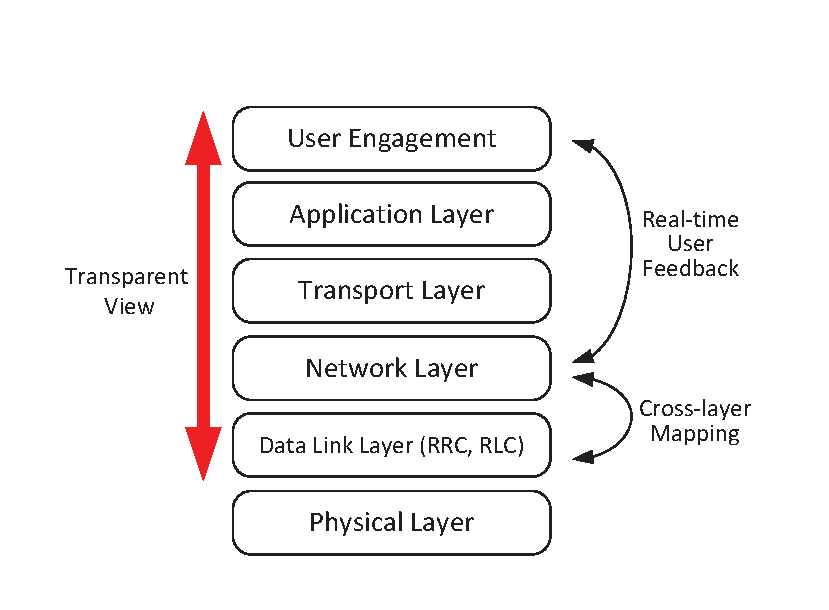
\includegraphics[width=0.5\textwidth]{figs/transLayer_overview.eps}
\caption{Overview architecture of \textit{TransLayer}}
\label{fig:translayer.overview}
\end{figure}

We show the overall design of \textit{TransLayer} in Figure~\ref{fig:translayer.overview}. The goal of \textit{TransLayer} is to provide a transparent view to mobile researchers, and assist them to identify the root causes of application performance problems in the cellular network. There are two essential parts in \textit{TransLayer}: a real-time user feedback collection tool and a cross-layer mapping tool. The real-time user feedback collection tool correlates user identified performance issues with the actual IP packets. The cross-layer mapping tool would utilize lower layer features to pinpoint the root causes.

Our contributions in this paper are:
\begin{itemize}
	\item
	We implemented a cross-layer analysis tool, as a part of \textit{TransLayer}, to correlate the upper layer performance problems with ground truth lower layer information. Our tool could achieve up to \textit{99.8\%} successful mapping from network layer to RLC layer PDU (Packet Data Unit), which is the smallest data transmission unit in RLC layer. To the best of our knowledge, the tool is the first implementation that enables cross-layer mapping between ground truth information from upper layer to the lower layer.
	\item
	We designed a simple real-time user feedback tool, as another part of \textit{TransLayer}, to allocate the ground truth application performance issues. The tool is generalized to apply to any applications to assist people studying QoE problems in cellular network.
	\item
	We performed root cause analysis to identify interference between control and data plane problem that could potentially downgrade application performance. The root cause could be a direction for ISP (Internet Service Provider) to improve the cellular performance by modifying the implementation in Node B or eNB.
\end{itemize}

The paper is organized as follows. \S~\ref{sec:background} takes a brief overview on background knowledge of cellular network. \S~\ref{sec:challenge} highlights the potential challenges in developing \textit{TransLayer}. \S~\ref{sec:crossAnalysis} explains the cross-layer mapping mechanism, and \S~\ref{sec:feedback} describes the design of the real-time user feedback collection tool. \S~\ref{sec:eval} presents a case study of root cause analysis on abnormal RRC state transition problem. \S~\ref{sec:future} lists the future work for \textit{TransLayer}, and \S~\ref{sec:related} summarizes the related work in cross-layer analysis and QoE study.